\section{3D coordination algorithms}

\begin{frame}
	\frametitle{Motivation}
	\centering
	\href{mbzirc_video.mp4}{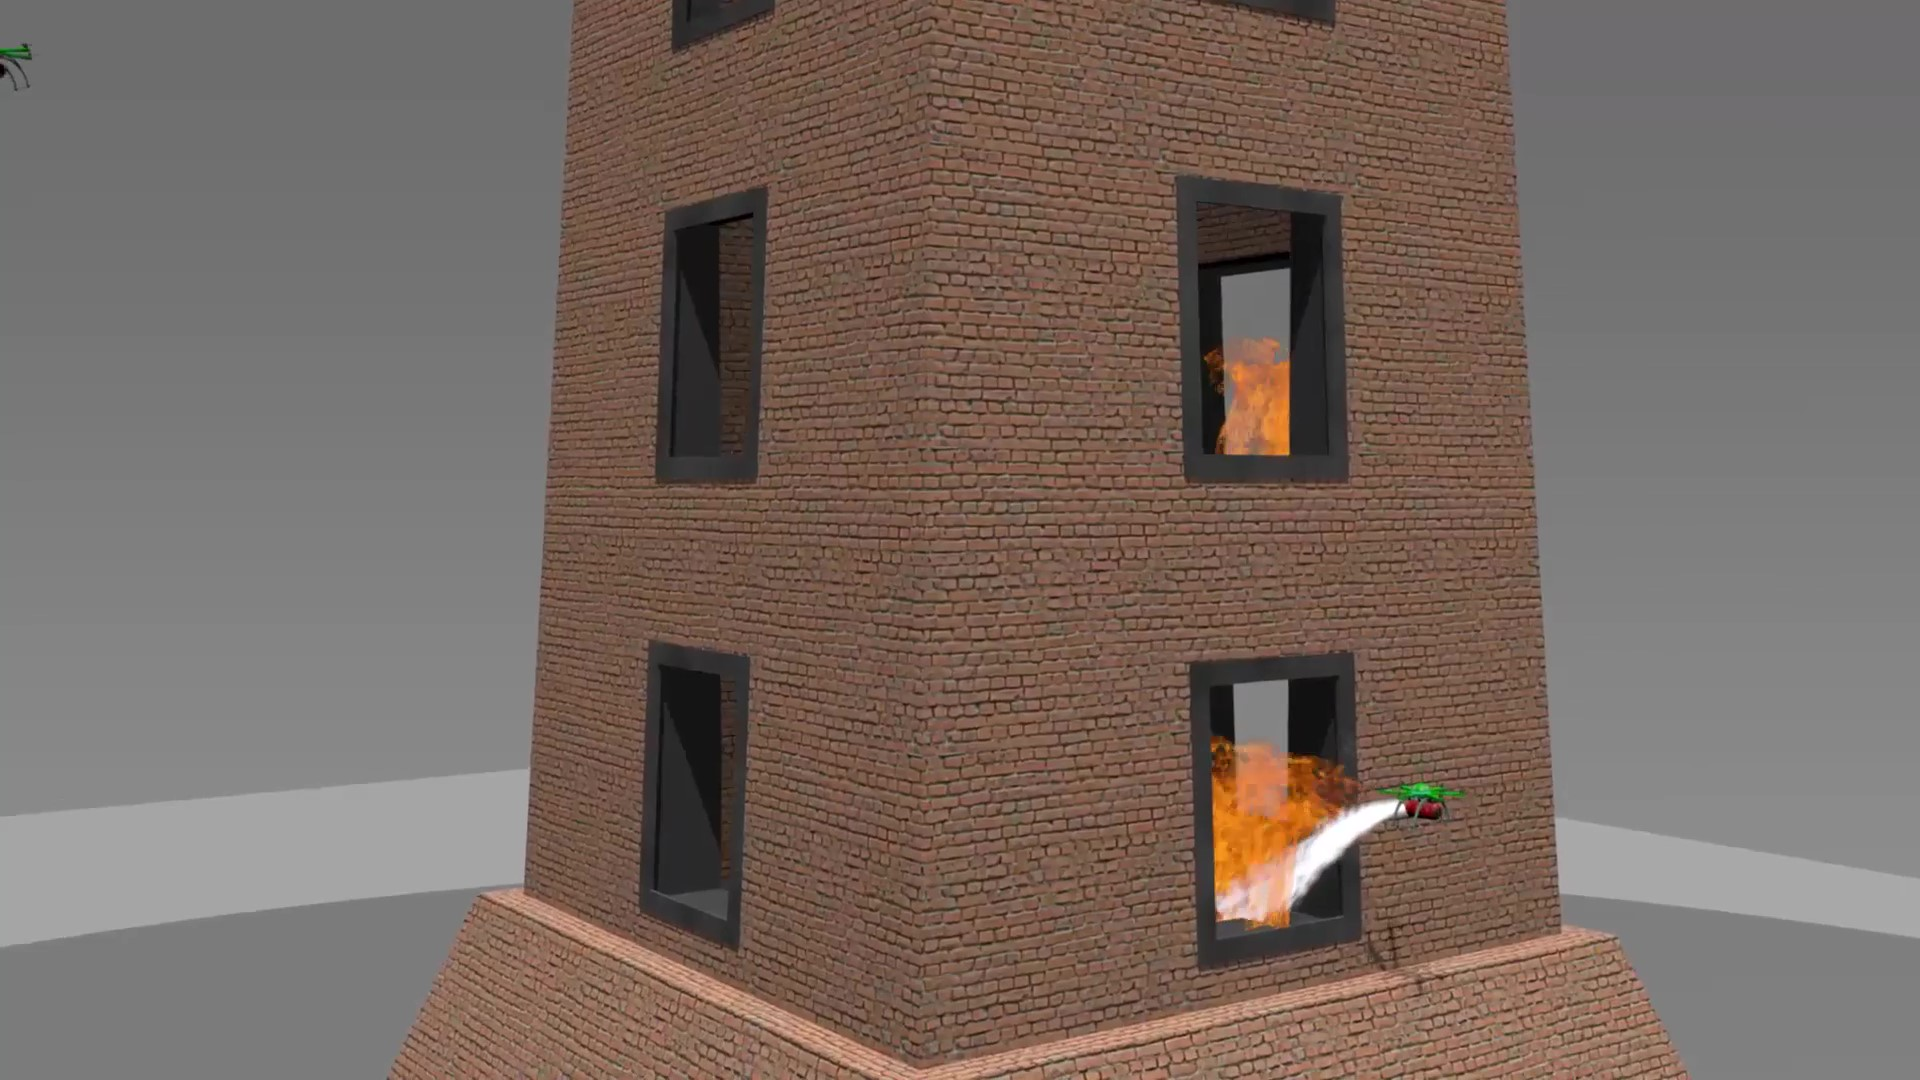
\includegraphics[width=0.8\textwidth]{figures/mbzirc_screen.jpg}}
	
\end{frame}

\subsection{Extension of 2D exploration solutions to 3D solution}
\begin{frame}
     \frametitle{Extension of 2D exploration solutions to 3D - single robot (1)}
     \begin{itemize}
     	\item[-] Reducing the dimension of the navigation space of robots\footcite{Bachrach2009}$\,$\footcite{Surmann2003}
     	\begin{itemize}
     		\item[-] 2.5D elevation maps 
     		%\item[-] Resulting model would probably contain unexplored areas
     	\end{itemize}	
     	\item[-] A complete 3D exploration is proposed in 2013 by Dornhege\footcite{Dornhege2013}
%     	algorithm was tested on a 5-DOF manipulator with a workspace radius of one
%     	meter
     	 %(i.e., an extension of Next-Best-View method to 3D)
     	 	\begin{itemize}
     			\item[-] Can be applied only in small areas (\textbf{computational effort})
     	 	\end{itemize}
      	\item[-] Combination of 2D and 3D exploration strategies\footcite{Maurovic2014}
      	%based on next-best-view method and room detection (Maurovic\footcite{Maurovic2014})
      	\begin{itemize}
      		\item[-] The robot switches to 3D exploration while a room is detected
      		\item[-] Local maps of rooms
      		% are used to overcome the problem of computational effort and memory consumption
      	\end{itemize}		
     \end{itemize}   
\end{frame}

\begin{frame}
	\frametitle{Extension of 2D exploration solutions to 3D - single robot (2)}
	\begin{itemize}
		\item[-] Formalized extension of the \textbf{frontier-based exploration}\footcite{ShadeNewman2011}
		\item[-] Next-best-view approach for 3D exploration\footcite{Bircher2016}
		
%		Shade and Newmann formalize, in [15], the 3D extension of
		%the frontier-based exploration. In particular, 3D frontiers are integrated with a
		%vector field approach to achieve 3D exploration with a stereo camera. 
		%3D requires highmemory and computational consumptions
		\item[-] Extraction of 3D frontiers from the OctoMap\footcite{Zhu2015}
%		\begin{itemize}
%			\item[-] Extract the 3D	frontiers from the OctoMap
%		\end{itemize}
		\item[-] 3D exploration based on surface frontier voxels \footcite{Senarathne2016} 
		\begin{figure}
			\centering
			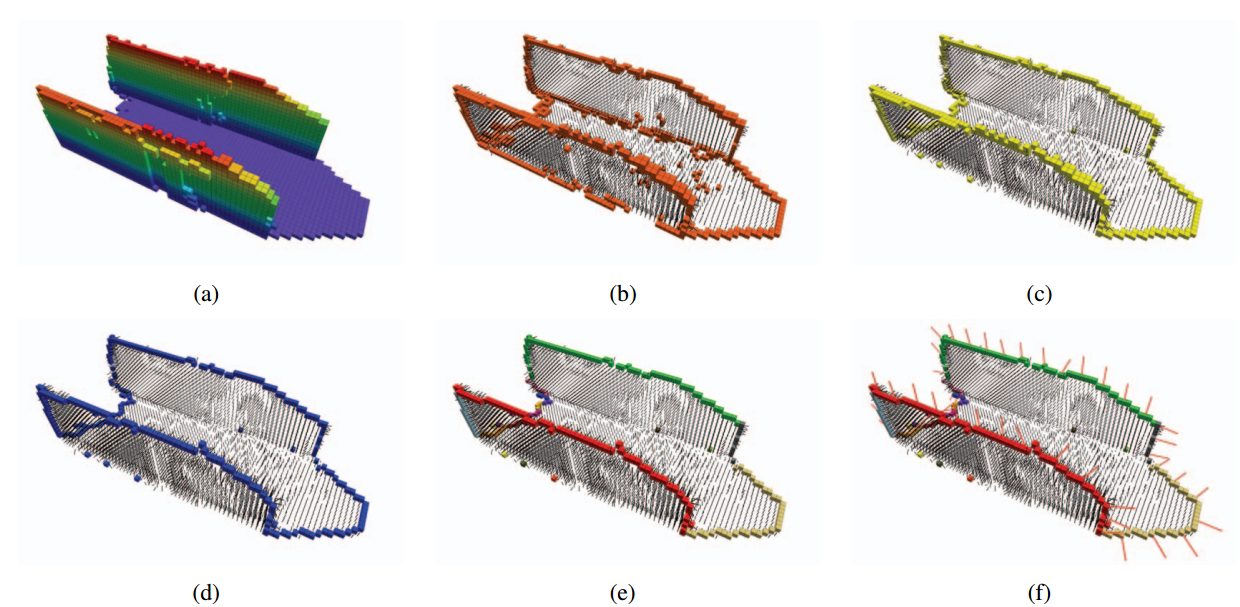
\includegraphics[width=0.4\textwidth]{figures/senarathne}
		\end{figure}
		
%presented an alternative approach to 3D exploration based on surface frontier voxels. The strategy focuses on seeking the expansion of mapped surfaces, instead of reducing unmapped voxels.
		
	\end{itemize}	
\end{frame}
%Next-best-view approach in the process of building 3D model of a real object used without any a priori information about the environment was described in \cite{VasquezGomez2014}. The algorithm determines each view to reconstruct an arbitrary object. Furthermore, authors proposed a method to deal with the uncertainty in sensor positioning.
%Next-best-view approach for 3D exploration was presented by Bircher et. al. \cite{Bircher2016}. Authors presented a novel path planning algorithm for the autonomous exploration of an unknown area. The proposed planner finds the best branch in an online computed tree. The quality of the branch is determined by the amount of unmapped space that can be explored. The planner is capable of running online, onboard a robot with limited resources.
%\begin{frame}
%     \frametitle{Extension of 2D exploration solutions to 3D (3)}
%		\begin{itemize}
%			\item[-]  for indoor environment
%			\item[-] Frontiers are searched just on a subset of nodes, the changed cells\footcite{Keidar2012}
%			\item[-] Method suffers from local minima
%			\item[-] The application in uncluttered environments results in few uninformative frontiers
%		\end{itemize}
%\end{frame}

\begin{frame}
	\frametitle{3D frontier exploration}
	\begin{columns}
		\begin{column}{0.5\textwidth}\centering
			\begin{center}
				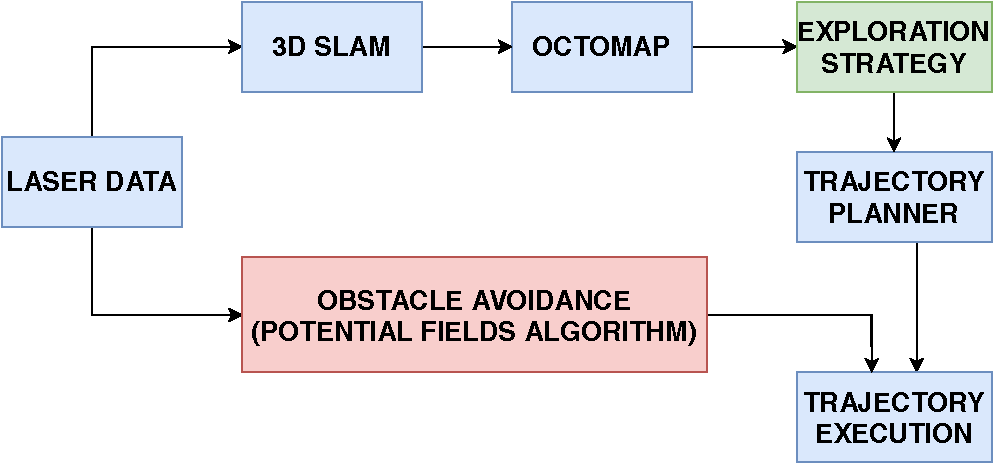
\includegraphics[height=3cm]{figures/3D_strategy}
				\label{fig:forest_uav}
			\end{center}
			%			\vspace{0.1cm}
			%			\begin{itemize}
			%				\item Stiff position-controlled
			%				\item Payload: 10-300 kg
			%				\item High speed, high accuracy
			%			\end{itemize}
		\end{column}
		\begin{column}{0.5\textwidth}\centering
			\begin{center}
				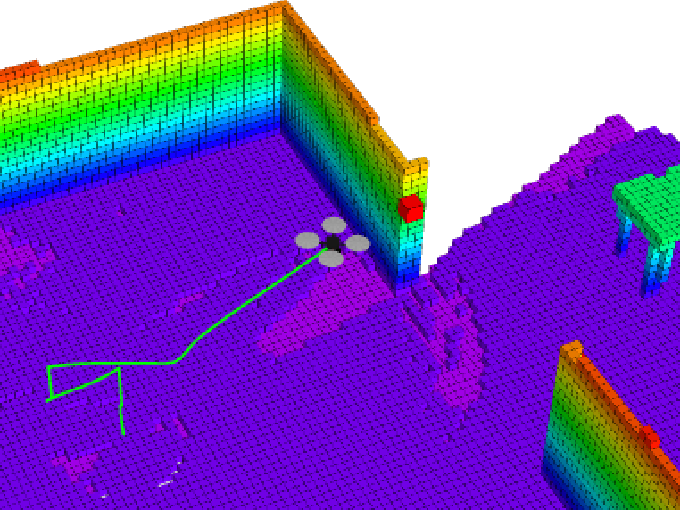
\includegraphics[height=3cm]{figures/octomap_and_drone}
				\label{fig:forest_plc}
			\end{center}
			%			\vspace{0.1cm}
			%			\begin{itemize}
			%				\item Joint torque-controlled
			%				\item Payload: up to 15 kg
			%				\item Environment sensing
			%			\end{itemize}
		\end{column}
	\end{columns}
\end{frame}